% Results and Evaluation

\chapter{نتایج و ارزیابی}\label{ch:5}
\section{مقدمه}\label{sec:5:1}
در این فصل دو روش \lr{KNN-LSTSVM} و \lr{RKNN-TSVM} به ترتیب در بخش‌های ‏\ref{sec:5:2} و ‏\ref{sec:5:3} به صورت جامع بررسی و ارزیابی می‌شود. این روش‌ها در دو بخش جداگانه مورد بررسی قرار گرفته‌اند. زیرا ایده و هدف اصلی این دو روش با یکدیگر متفاوت است. 
\begin{enumerate}
	\item هدف اصلی در روش \lr{KNN-LSTSVM} ضمن حفظ مزیت اصلی روش \lr{LSTSVM}، اضافه کردن گراف نزدیک‌ترین همسایه به منظور بهبود دقت این مدل است.
	\item 	روش \lr{RKNN-TSVM} با کمینه کردن ریسک ساختاری و شیوه جدید وزن‌دهی، دقت روش \lr{WLTSVM} را بهبود می‌دهد. با این حال در روش \lr{RKNN-TSVM}، افزایش سرعت آموزش هم مد نظر است.
\end{enumerate}

در ادامه عملکرد روش پیشنهادی از نظر دقت و سرعت روی مجموعه داده‌های مختلف سنجیده می‌شود.

\section{ارزیابی روش \lr{KNN-LSTSVM}}\label{sec:5:2}
ابتدا نحوه پیاده‌سازی و انتخاب پارامترهای بهینه توضیح داده شده است. سپس عملکرد روش \lr{KNN-LSTSVM} روی مجموعه داده‌های مصنوعی بررسی می‌شود. بطوریکه ناحیه تصمیم خطی و غیر خطی این روش در فضای دو بعدی نشان داده شده است. در آخر نتایج روی مجموعه داده‌های \lr{UCI} و \lr{NDC} مورد بحث قرار می‌گیرد.

\subsection{نحوه پیاده‌سازی و اجرای الگوریتم‌ها}\label{sec:5:2:1}
تمام روش‌ها در زبان برنامه‌نویسی پایتون\footnote{\lr{Python}}  \cite{ceder2010} پیاده‌سازی شده است. آزمایش‌ها روی یک کامپیوتر شخصی با پردازنده \lr{Core i7 6700K}، سیستم عامل \lr{Windows 8} و 32 گیگابایت حافظه صورت گرفته است. اعمال جبر خطی با کتابخانه \lr{NumPy} \cite{walt2011} انجام شده است. همچنین کتابخانه \lr{SciPy} \cite{jones2014} برای محاسبه فاصله و توابع آماری بکار گرفته شده است. همچنین الگوریتم بهینه‌سازی \lr{clipDCD} جهت بهبود سرعت اجرا، در \lr{Cython} \cite{behnel2011} پیاده‌سازی شده است.

دقت روش \lr{TSVM} و گسترش‌هایش به انتخاب پارامترهای بهینه بسیار وابسته است. بدین منظور جستجوی شبکه‌ای\footnote{\lr{Grid search}}  برای پیدا کردن پارامترهای بهینه استفاده می‌شود. همچنین تابع \lr{TSVM} را به عنوان تابع هسته  $k(x_i, x_j)=\exp({-\left\|x_i - x_j\right\|^2}/\gamma^2)$ اغلب بکار می‌گیرند. پارامترهای خطا در روش‌های \lr{TSVM}، \lr{WLTSVM}، \lr{LSTSVM} و \lr{KNN-LSTSVM} از مجموعه  $\{2^i \mid i=-10, -9, \dots, 9, 10\}$ انتخاب شده است.  پارامتر تابع هسته $\gamma$  نیز از مجموعه  $\{2^i \mid i=-15, -14, \dots, 5\}$ تعیین می‌شود. تعداد نزدیک‌ترین همسایه  $k$ از مجموعه  $\{2,3, \dots, 10\}$ انتخاب می‌گردد.

\subsection{مجموعه داده مصنوعی}\label{sec:5:2:2}
به منظور نشان دادن برتری روش \lr{KNN-LSTSVM} نسبت به روش \lr{LSTSVM} به صورت هندسی، آزمایش روی مجموعه داده \lr{Ripley}  \cite{ripley2007} و \lr{Checkerboard} \cite{ho1996} انجام گرفته است که به ترتیب شامل 250 و 1000 نمونه آموزشی هستند. شکل ‏\ref{fig:LSTSVM-vs-KNN-LSTSVM-R} و شکل \ref{fig:LSTSVM-vs-KNN-LSTSVM-C} عملکرد و ناحیه تصمیم روش \lr{LS-TSVM} و \lr{KNN-LSTSVM} را به ترتیب برای روی مجموعه داده \lr{Ripley} و \lr{Checkerboard} نشان می‌دهد.

همانطور که در شکل ‏\ref{fig:LSTSVM-vs-KNN-LSTSVM-R} و شکل ‏\ref{fig:LSTSVM-vs-KNN-LSTSVM-C} نشان داده شده است، روش پیشنهادی \lr{KNN-LSTSVM} دقت بیشتر و ناحیه تصمیم بهتری دارد. بطوریکه تعداد نمونه‌های تست کمتری به طور اشتباه دسته‌بندی شده‌اند. به عبارت دیگر، تعمیم‌پذیری روش \lr{KNN-LSTSVM} بیشتر است.

\begin{figure}[!t]
	\centering
	\subfloat[\lr{LSTSVM} (\lr{$C=2^{-10}, \gamma=2^{1}$})]{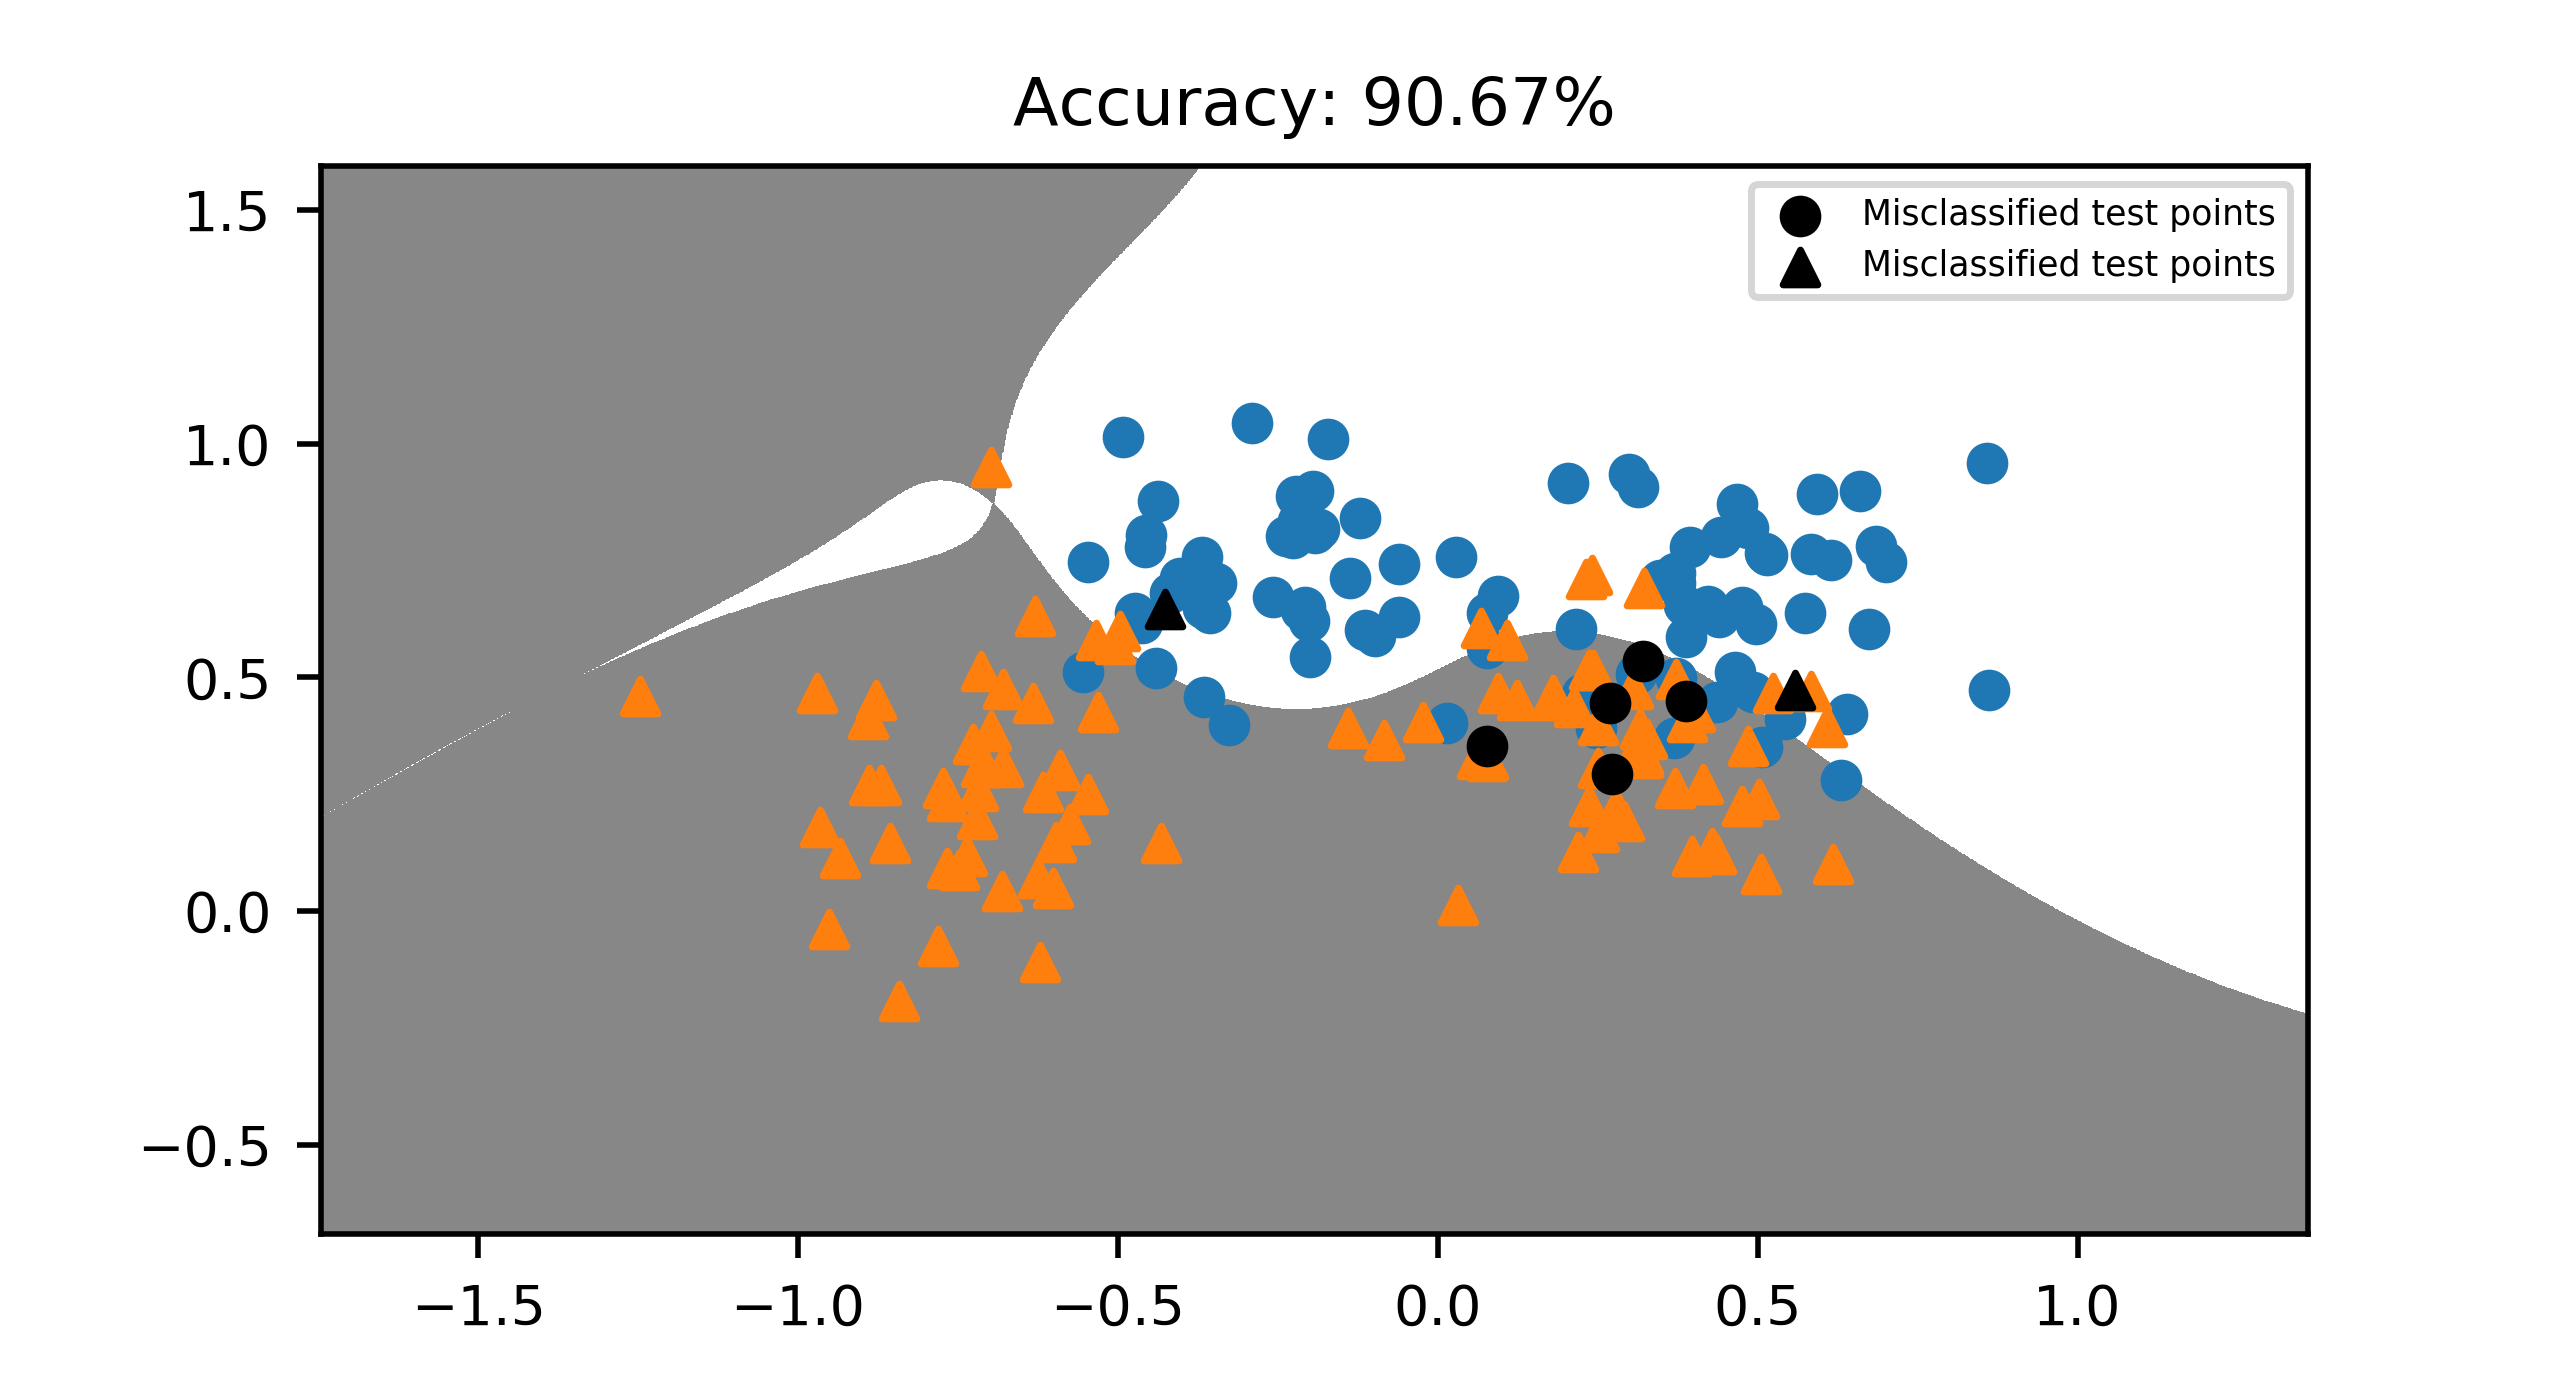
\includegraphics[width=0.5\textwidth]{LSTSVM-Ripley}}
	\subfloat[\lr{KNN-LSTSVM} \lr{($C=2^{-7}, k=6, \gamma=1$)}]{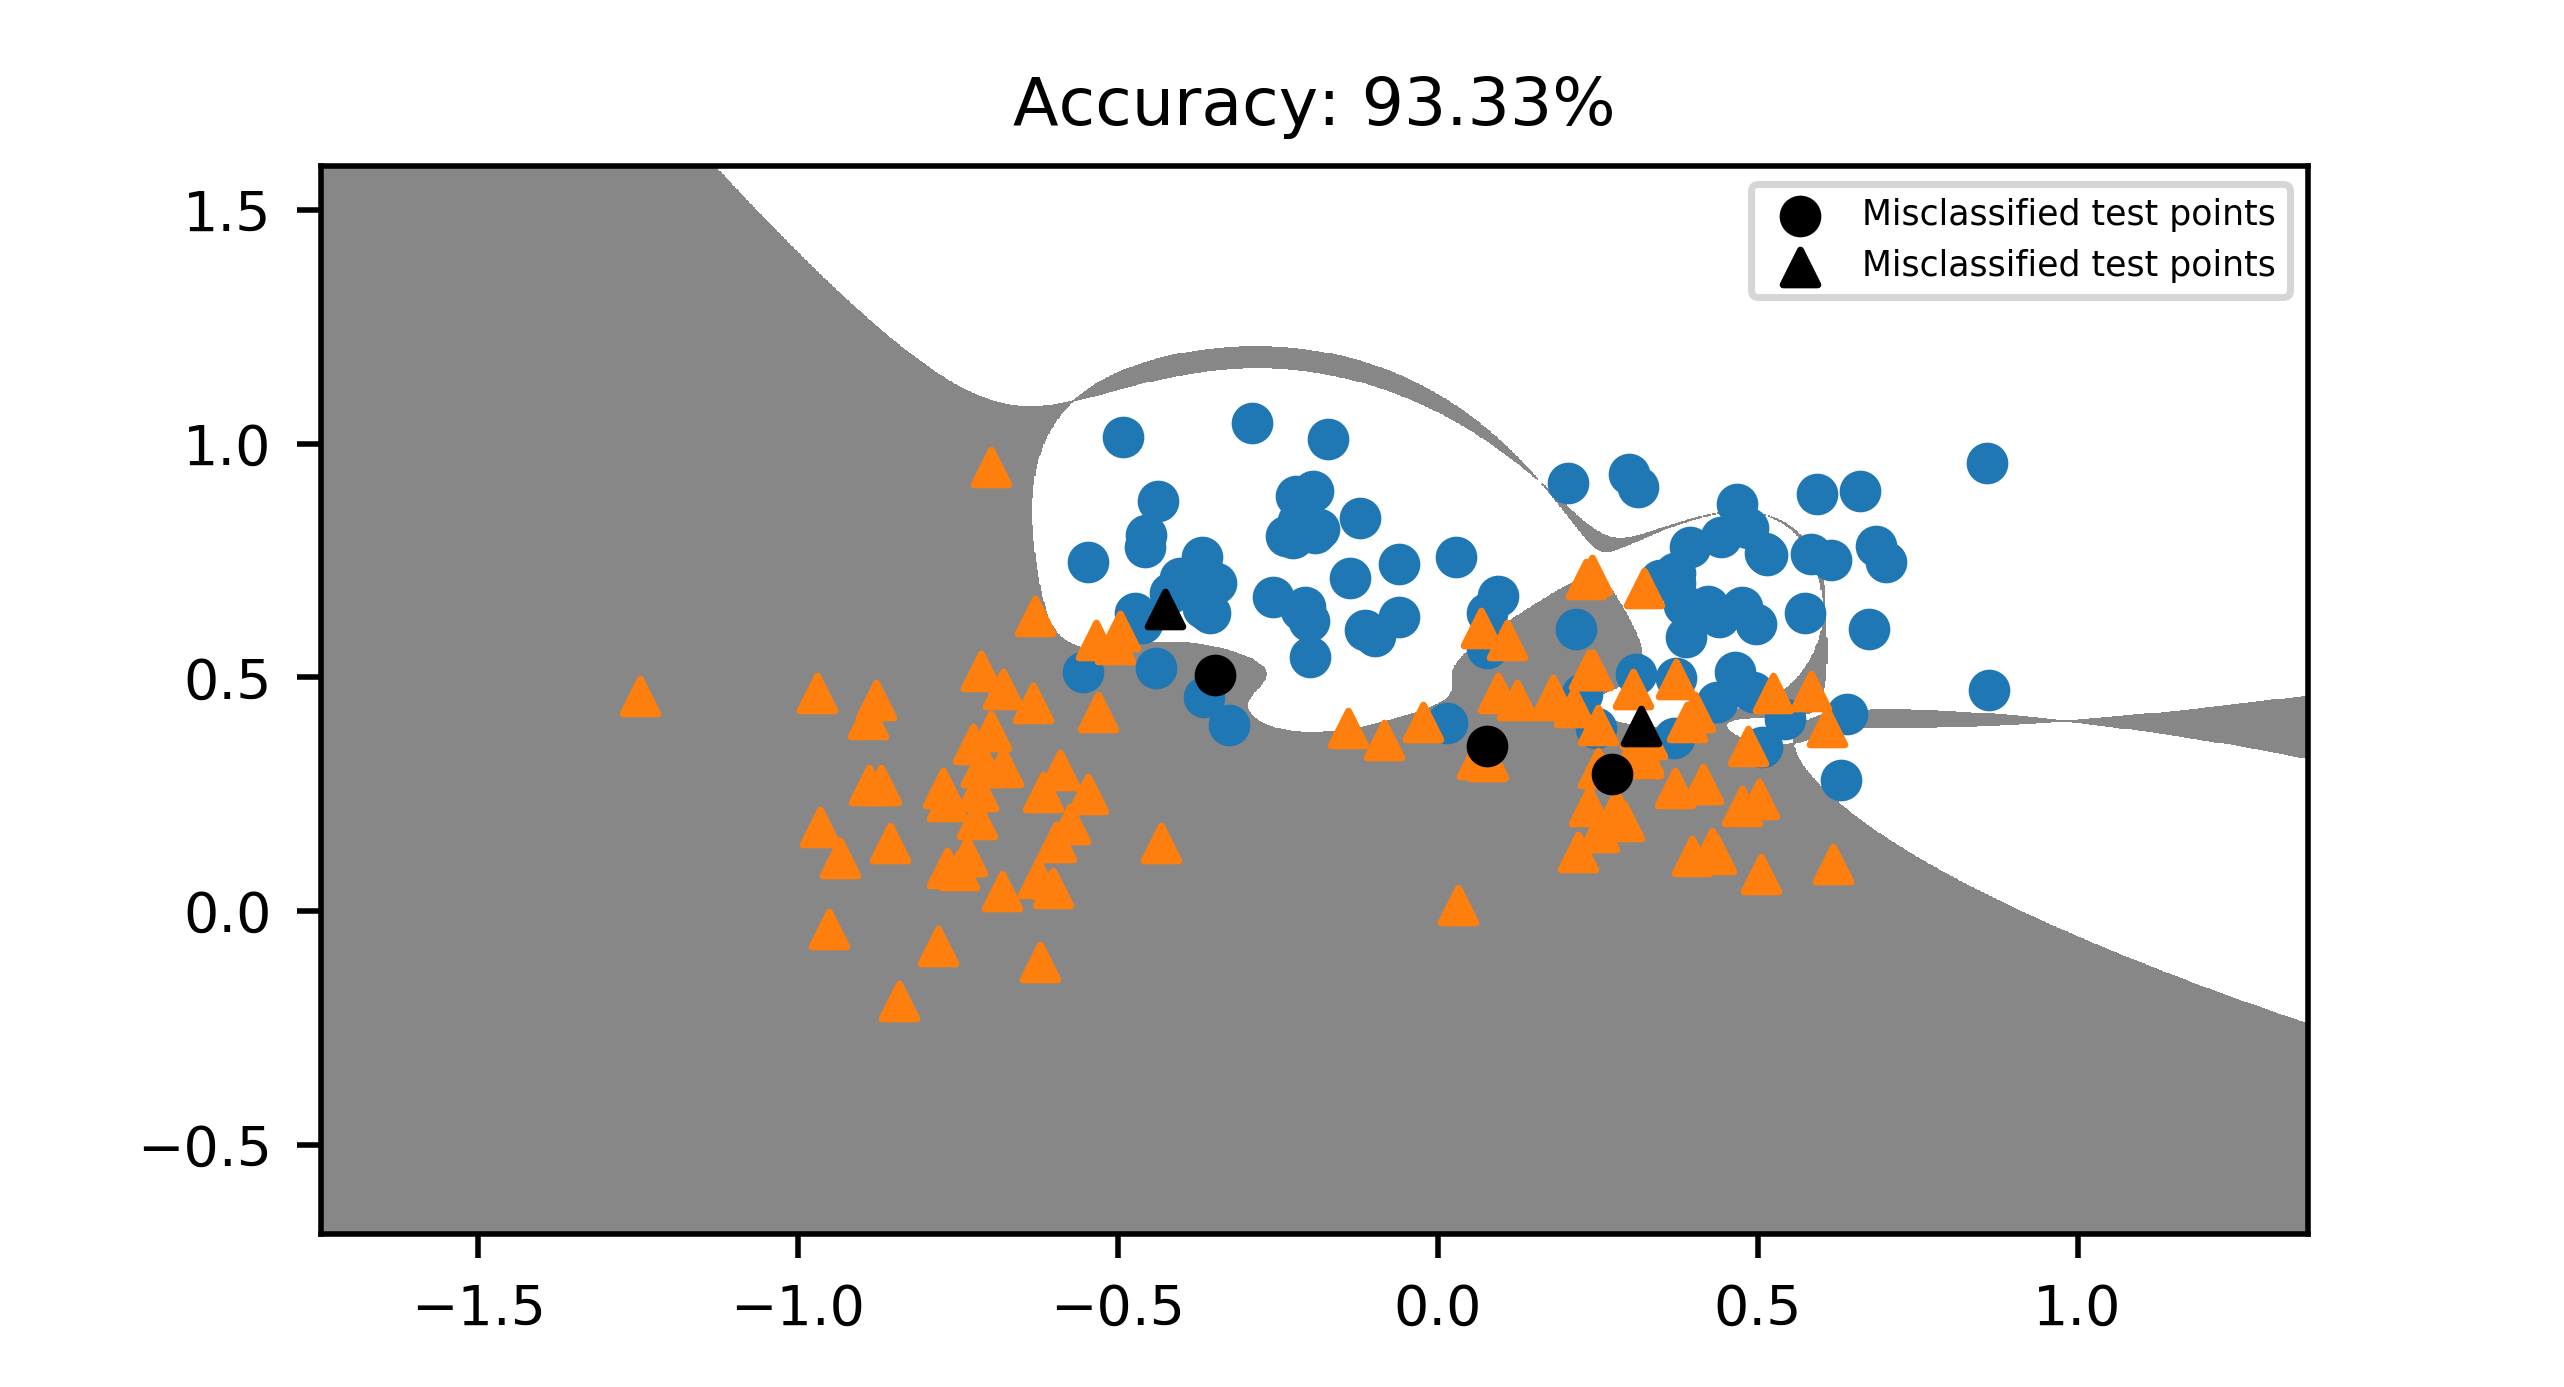
\includegraphics[width=0.5\textwidth]{KNN-LSTSVM-Ripley}}
	\caption{عملکرد و ناحیه تصمیم روش  \lr{LS-TSVM} و  \lr{KNN-LSTSVM} را برای روی داده  \lr{Ripley}}
		\label{fig:LSTSVM-vs-KNN-LSTSVM-R}
\end{figure}

\begin{figure}[!ht]
	\centering
	\subfloat[\lr{LSTSVM} (\lr{$C=2^{-10}, \gamma=2^{1}$})]{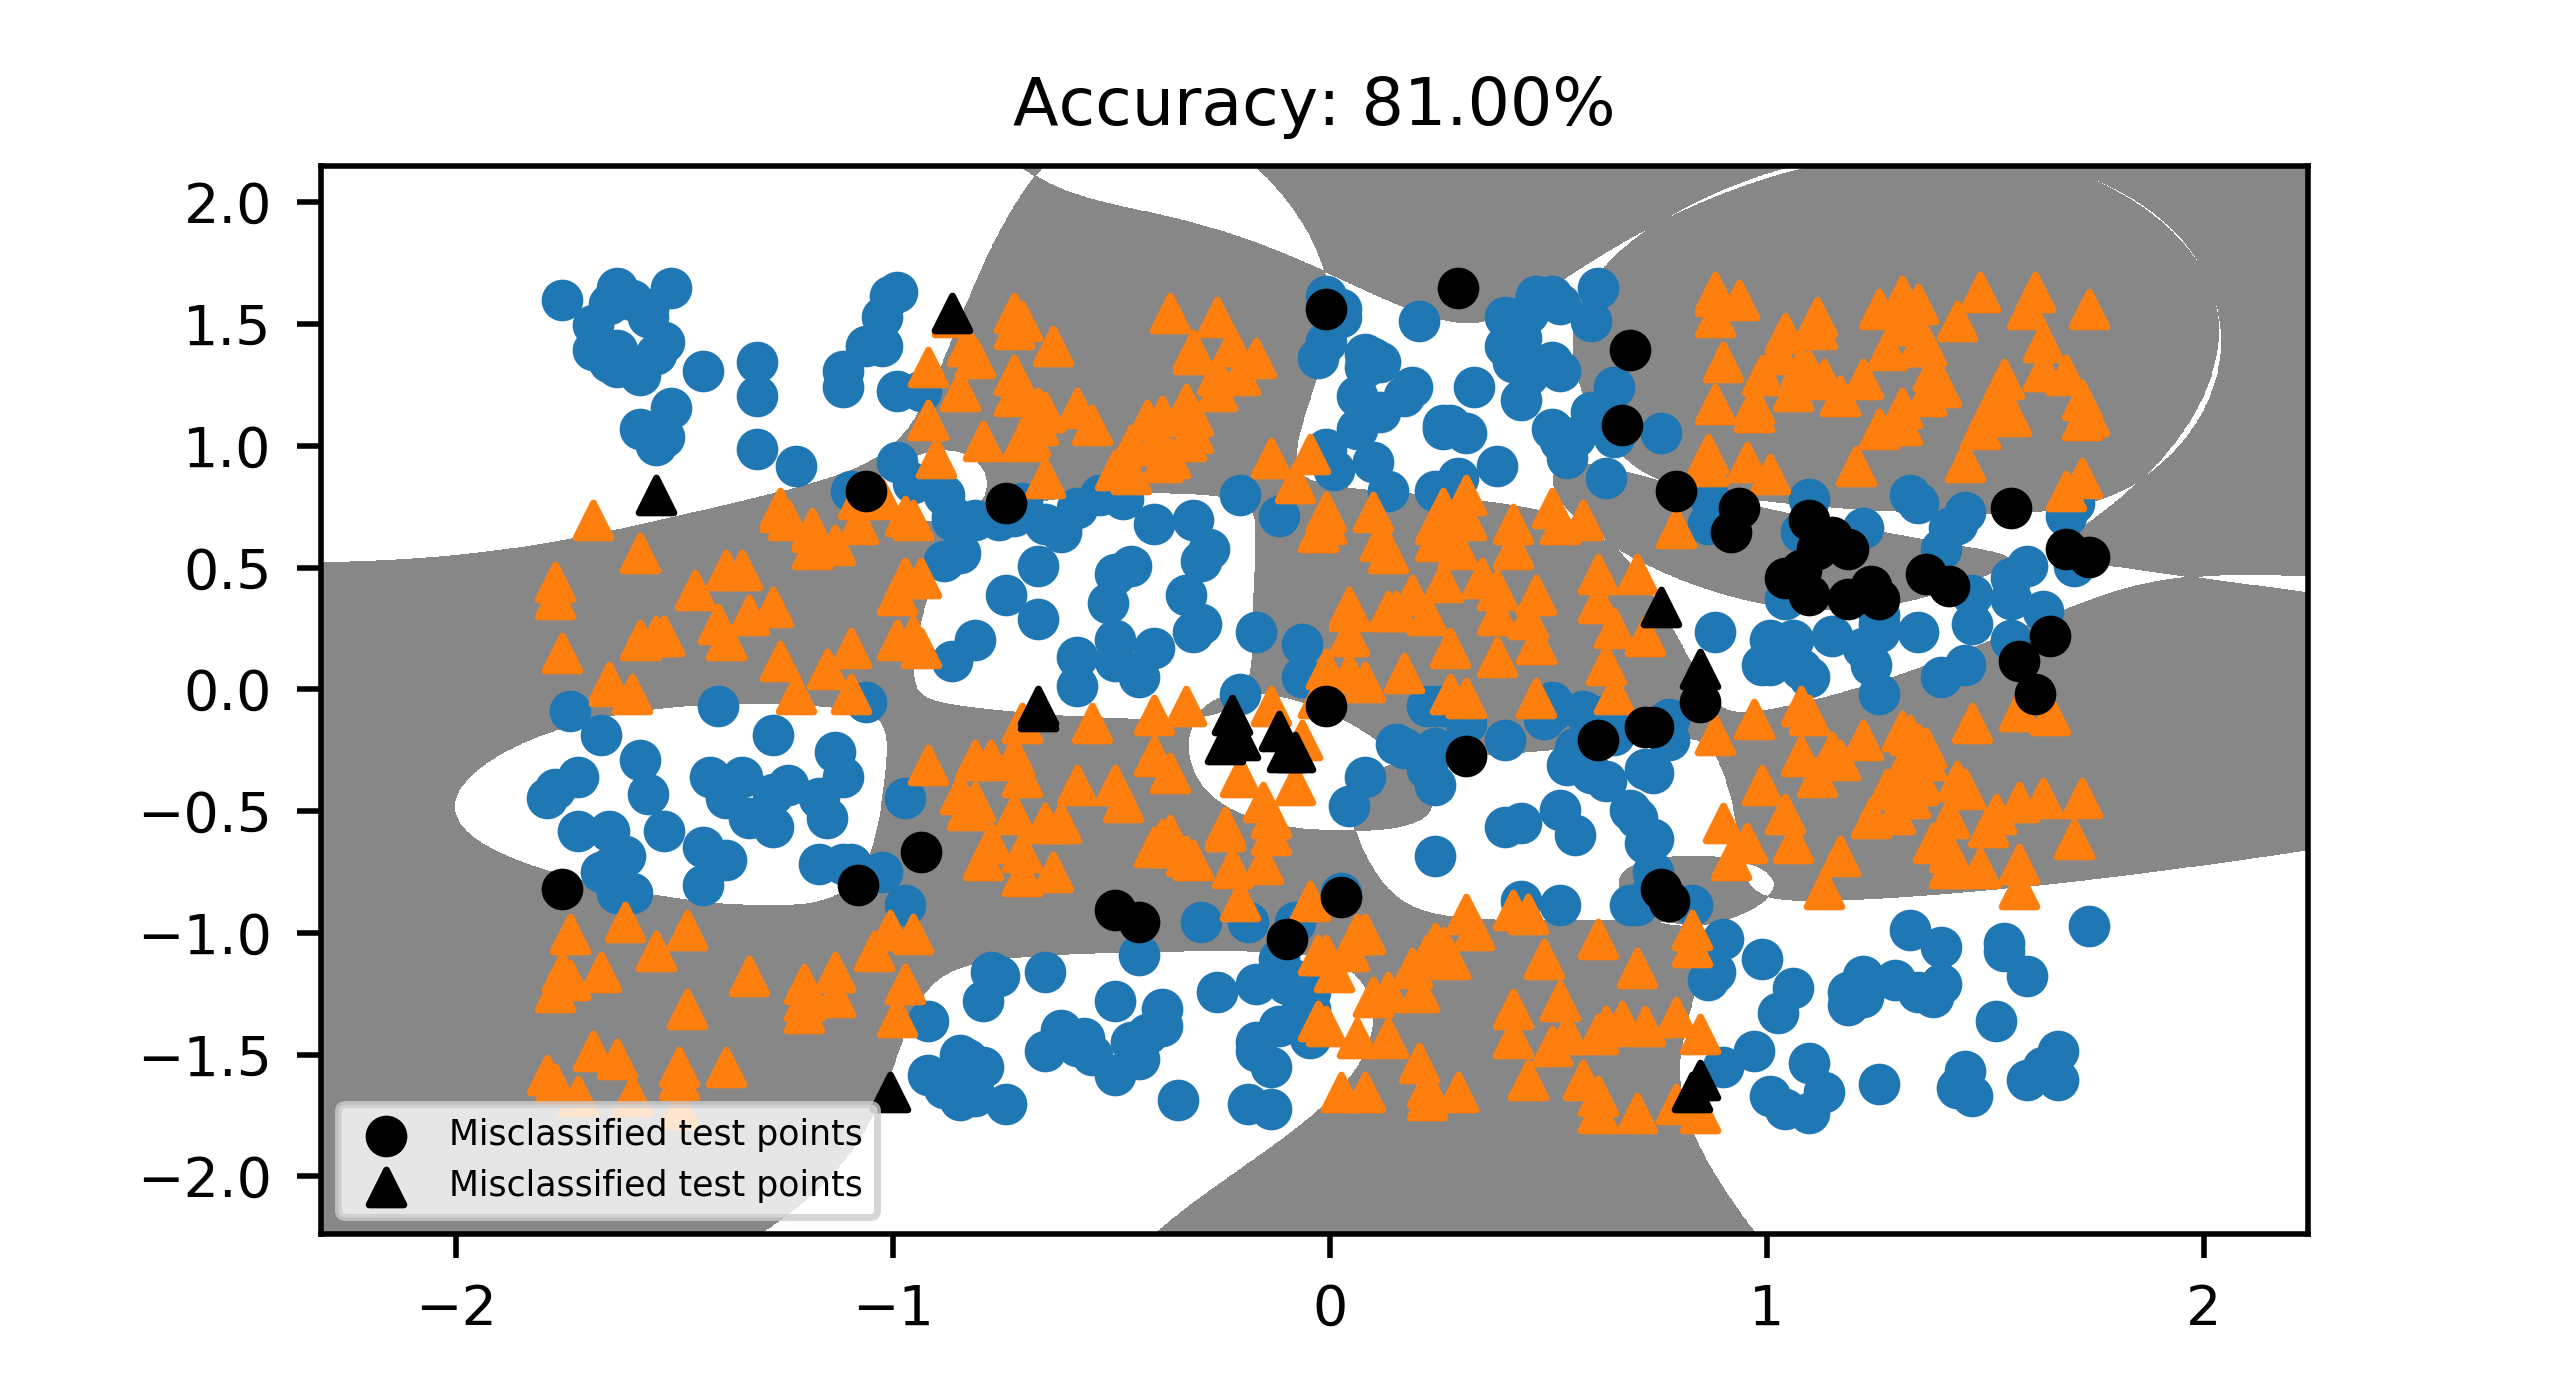
\includegraphics[width=0.5\textwidth]{LSTSVM-check}}
	\subfloat[\lr{KNN-LSTSVM} \lr{($C=2^{-10}, k=6, \gamma=2^{1}$)}]{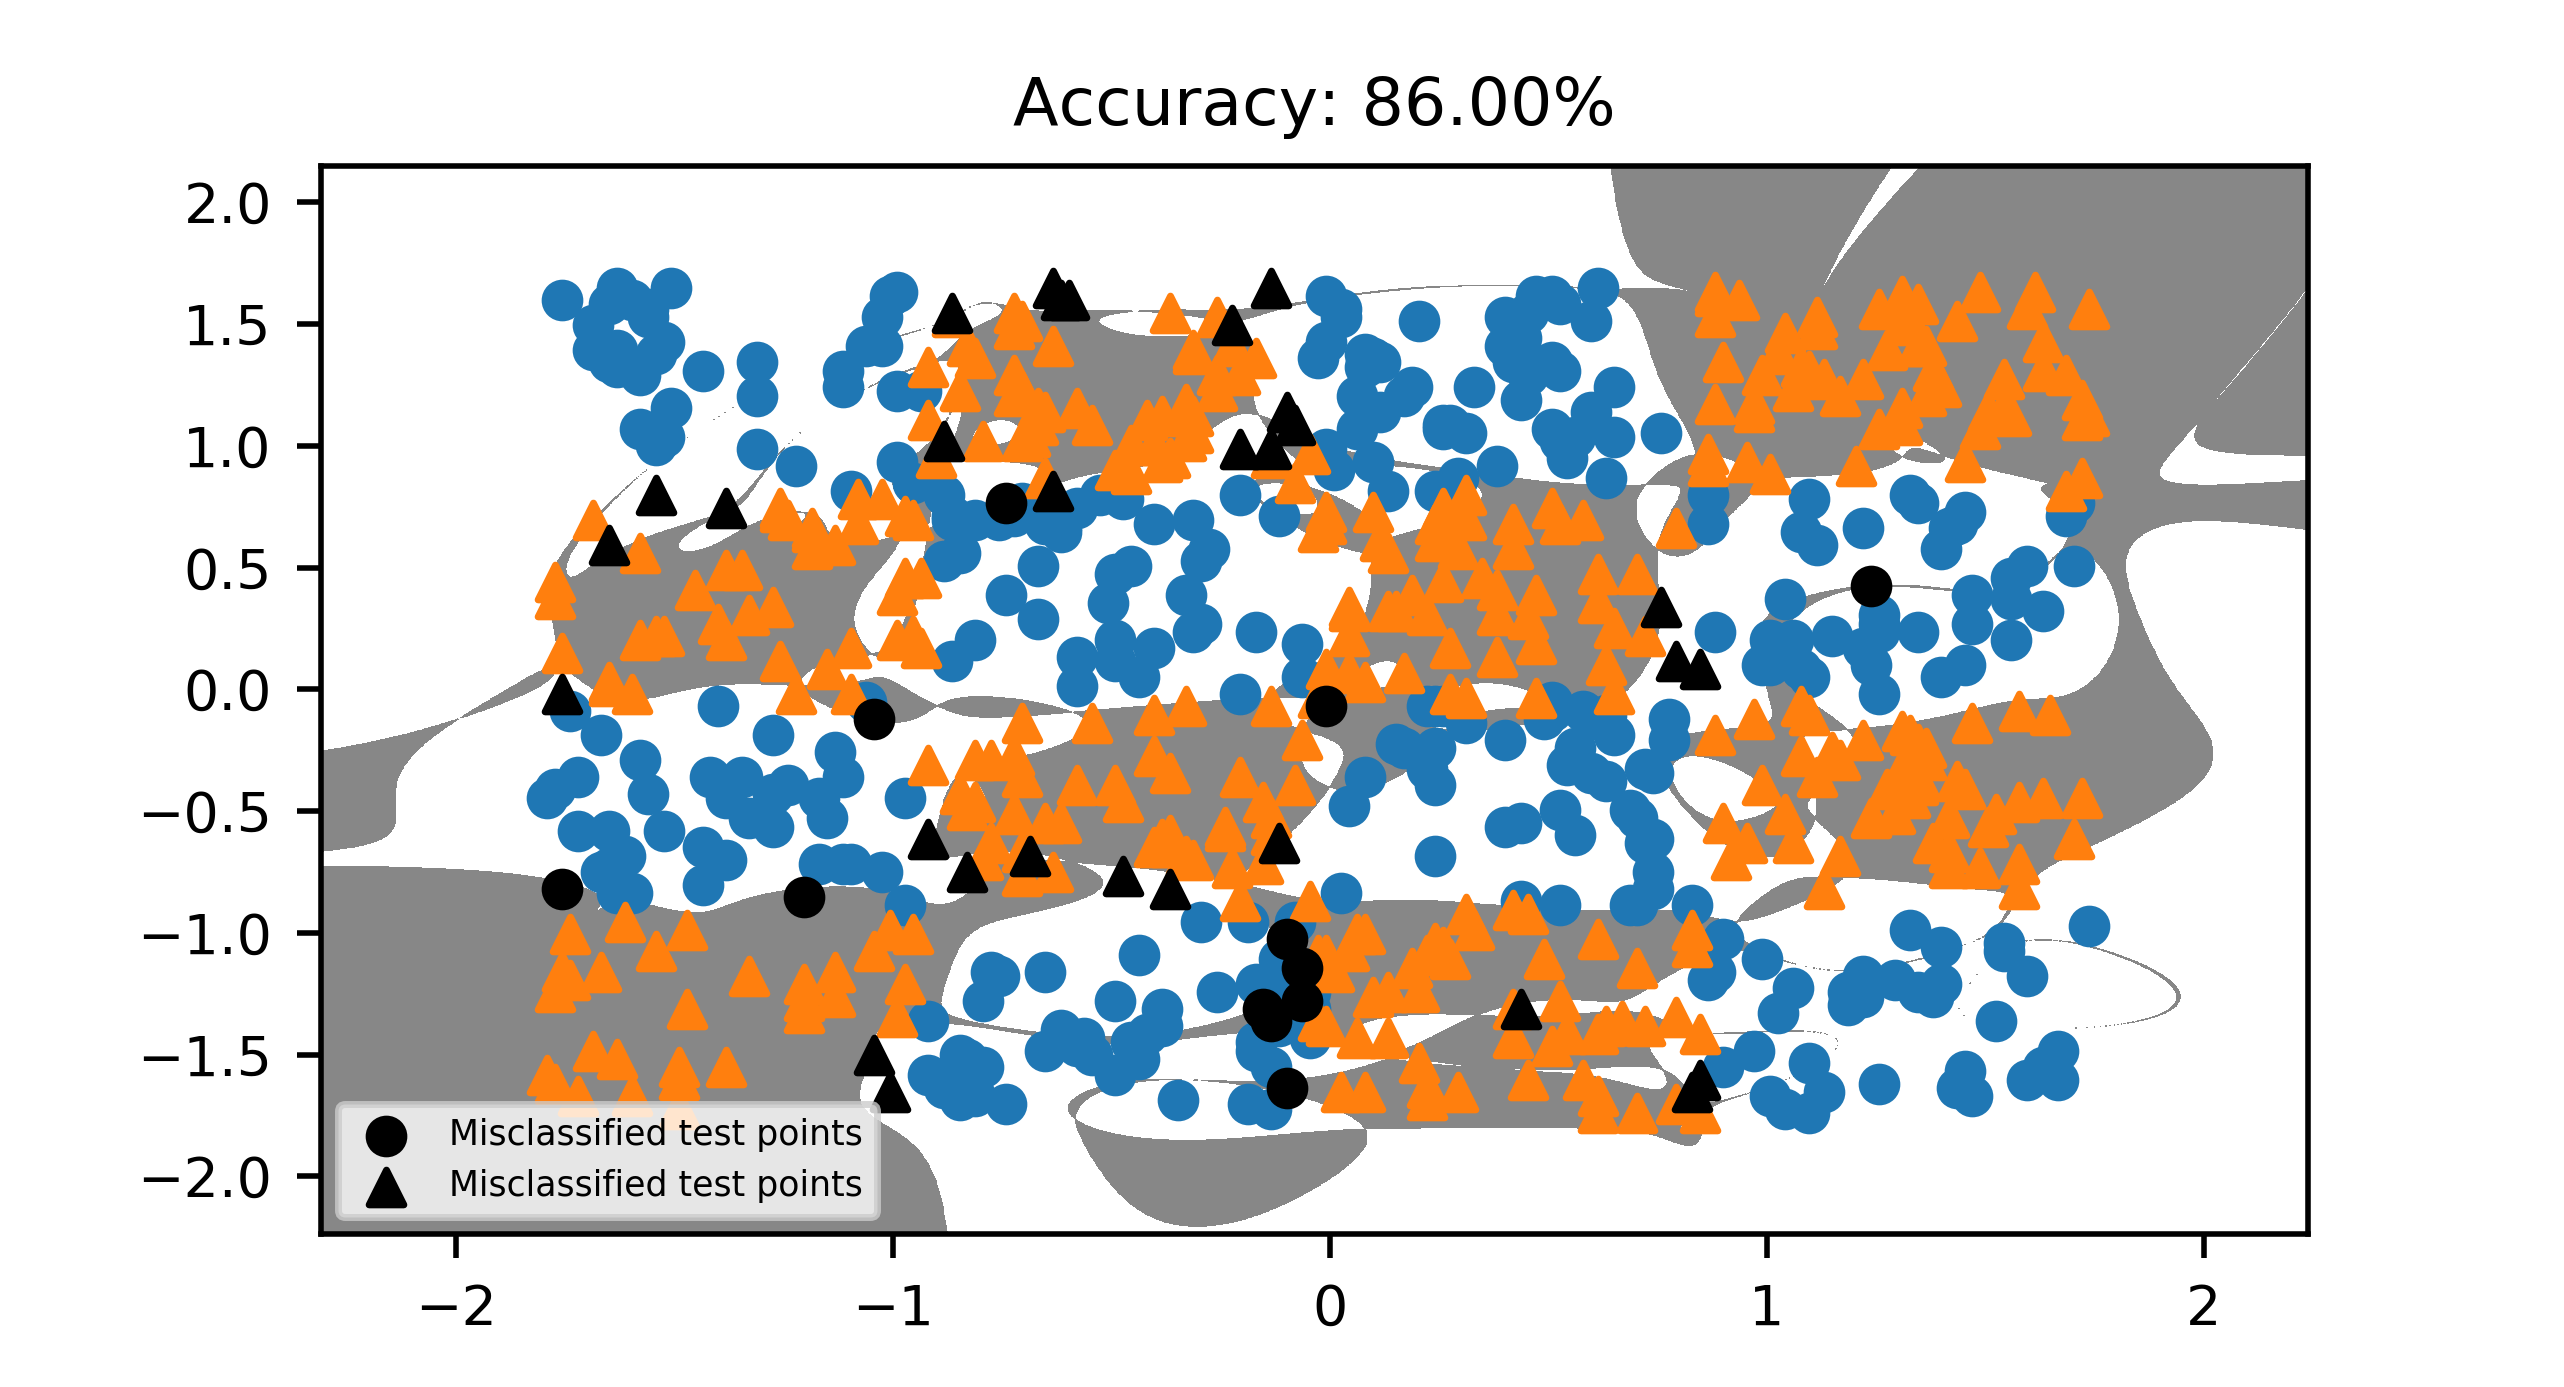
\includegraphics[width=0.5\textwidth]{KNN-LSTSVM-check}}
	\caption{عملکرد و ناحیه تصمیم روش  \lr{LS-TSVM} و  \lr{KNN-LSTSVM} را برای روی داده  \lr{Checkerboard}}
	\label{fig:LSTSVM-vs-KNN-LSTSVM-C}
\end{figure}

\newpage

\subsection{نتایج ارزیابی بر روی مجموعه داده \lr{UCI}}\label{sec:5:2:3}
در این زیر بخش، عملکرد روش \lr{KNN-LSTSVM} روی 14 مجموعه داده از مخرن  \lr{UCI}\footnote{\lr{https://archive.ics.uci.edu/ml/index.php}} ارزیابی و بررسی می‌شود. مشخصات این مجموعه داده‌ها در جدول \ref{tab:1} ذکر شده است.

\begin{table}[!t]
	\centering
	\caption{مشخصات مجموعه داده‌ها برای ارزیابی روش \lr{KNN-LSTSVM}}
	%\tabcolsep=0.11cm
	\begin{tabular}{l c c c c}
		\hline
		% after \\: \hline or \cline{col1-col2} \cline{col3-col4} ...
		مجموعه داده & تعداد نمونه‌ها & نمونه‌های مثبت & نمونه‌های منفی &تعداد ویژگی‌ها \\
		\hline
	\lr{{Austrailian}} & {690} & {307} & {383} & {14} \\
	\lr{{Bupa-Liver}} & {345} & {145} & {200} & {6} \\
	\lr{{Cleveland}} & {303} & {139} & {164} & {13} \\
	\lr{{Haber-Man}} & {306} & {225} & {81} & {3} \\
	\lr{{Heart-Statlog}} & {270} & {120} & {150} & {13} \\
	\lr{{Hepatits}} & {155} & {32} & {123} & {19} \\
	\lr{{Ionsphere}} & {351} & {225} & {126} & {34} \\
	\lr{{Monk3}} & {554} & {288} & {266} & {6} \\
	\lr{{Pima-Indian}} & {768} & {268} & {500} & {8} \\
	\lr{{Sonar}} & {208} & {97} & {111} & {60} \\
	\lr{{Titanic}} & {891} & {342} & {549} & {7} \\
	\lr{{Votes}} & {435} & {267} & {168} & {16} \\
	\lr{{Wdbc}} & {569} & {212} & {357} & {30} \\
	\lr{{Wpbc}} & {198} & {47} & {151} & {33} \\
		\hline
	\end{tabular}
	
	\label{tab:1}
\end{table}

دقت دسته‌بندی هر کدام از روش‌ها توسط معیار ارزیابی اعتبارسنج ضربدری  ۱۰تایی سنجیده می‌شود. بطوریکه نمونه‌های آموزشی به صورت تصادفی به 10 بخش تقیسم می‌شوند. یکی از این بخش‌ها به عنوان نمونه‌های تست در نظر گرفته می‌شود و سایر بخش‌ها برای آموزش دسته‌بند استفاده می‌گردد. این فرآیند 10 بار تکرار می‌شود تا زمانی که تمام بخش‌ها به عنوان نمونه تست استفاده شود \cite{bishop2006}.

جدول ‏5 2 میانگین و انحراف معیار دقت (به درصد) را برای دسته‌بندهای \lr{TSVM}، \lr{WLTSVM}، \lr{LSTSVM} و \lr{KNN-LSTSVM }نشان می‌دهد. همچنین زمان آموزش دسته‌بندها (به ثانیه) و مقادیر بهینه ‍پارامترها نیز در جدول ‏\ref{tab:3} درج شده است. لازم به ذکر است که محاسبه گراف نزدیک‌ترین همسایه در زمان آموزش دسته‌بندهای \lr{WLTSVM} و \lr{KNN-LSTSVM} لحاظ شده است. 

\begin{table*}[!t]
	\small
	\centering
	\caption{مقایسه دقت و زمان آموزش دسته‌بندهای \lr{TSVM}، \lr{WLTSVM}،  \lr{LSTSVM} و \lr{KNN-LSTSVM}}
	\ra{1.3} % Space between rows
	\tabcolsep=0.13cm % Adjusts column width
	\begin{tabular}{p{2.0cm} p{1.95cm} p{1.1cm} c p{1.95cm} p{1.1cm} c p{1.95cm} p{1.1cm} c p{1.95cm} p{1.1cm}}
		\toprule
		
		% after \\: \hline or \cline{col1-col2} \cline{col3-col4} ...
		مجموعه داده & \multicolumn{2}{c}{\lr{TSVM}} && \multicolumn{2}{c}{\lr{WLTSVM}} && \multicolumn{2}{c}{\lr{LSTSVM}} && \multicolumn{2}{c}{\lr{KNN-LSTSVM}} \\
		\cmidrule{2-3} \cmidrule{5-6} \cmidrule{8-9} \cmidrule{11-12}
		($m\times n$) & دقت (\%) & زمان اجرا && دقت (\%) & زمان اجرا && دقت (\%) & زمان اجرا &&  دقت (\%) & زمان اجرا \\
		& $(C_1, C_2, \gamma)$  &  && $(C_, \gamma, k)$ &  && $(C_1, C_2, \gamma)$  &  && $(C, \gamma, k)$  &  \\
		\midrule
		\lr{Australian} & \textbf{$87.97\pm2.75$} & $0.070$ && $87.25\pm3.65$ & $0.264$ && $87.68\pm3.79$ & $0.058$ &&  $87.39\pm3.31$ & $0.230$ \\
		($690\times 14$) & ($2^{-4}, 2^{-4}, 2^{-6}$) &  && ($2^{-1}, 2^{-14}, 6$) &  && ($2^{-7}, 2^{-5}, 2^{-6}$) &  && ($2^{3}, 2^{-13}, 7$) &  \\
		\lr{Bupa-Liver} & $73.62\pm4.77$ & $0.082$ && $74.82\pm3.84$ & $0.193$ && $74.51\pm6.89$ & $0.007$ &&  \textbf{$75.96\pm5.40$} & $0.041$ \\
		($345\times 6$) & ($2^{-3}, 2^{-3}, 2^{-6}$) &  && ($2^{2}, 2^{-7}, 4$) &  && ($2^{5}, 2^{4}, 2^{-6}$) &  && ($2^{10}, 2^{-6}, 7$) &  \\
		\lr{Cleveland} & $84.86\pm3.76$ & $0.037$ && $84.48\pm6.29$ & $0.082$ && $85.49\pm4.92$ & $0.005$ &&  \textbf{$85.51\pm6.41$} & $0.026$ \\
		($303\times 13$) & ($2^{0}, 2^{-1}, 2^{-11}$) &  && ($2^{3}, 2^{-9}, 7$) &  && ($2^{2}, 2^{1}, 2^{-11}$) &  && ($2^{-2}, 2^{-15}, 5$) &  \\
		\lr{Haber-Man} & $76.14\pm3.60$ & $0.082$ && $75.80\pm5.22$ & $0.138$ && $76.73\pm7.83$ & $0.005$ &&  \textbf{$76.81\pm5.82$} & $0.031$ \\
		($306\times 3$) & ($2^{1}, 2^{-1}, 2^{-9}$) &  && ($2^{3}, 2^{-4}, 2$) &  && ($2^{9}, 2^{9}, 2^{-7}$) &  && ($2^{-10}, 2^{-9}, 9$) &  \\
		\lr{Heart-Statlog} & \textbf{$85.56\pm5.84$} & $0.041$ && $85.19\pm5.49$ & $0.032$ && $85.19\pm6.20$ & $0.004$ &&  $85.19\pm5.74$ & $0.022$ \\
		($270\times 13$) & ($2^{1}, 2^{0}, 2^{-11}$) &  && ($2^{1}, 2^{-13}, 6$) &  && ($2^{0}, 2^{-1}, 2^{-12}$) &  && ($2^{-1}, 2^{-14}, 7$) &  \\
		\lr{Hepatits} & $85.79\pm8.65$ & $0.003$ && $86.50\pm8.79$ & $0.040$ && \textbf{$87.79\pm6.57$} & $0.001$ &&  $87.13\pm7.59$ & $0.006$ \\
		($155\times 19$) & ($2^{-4}, 2^{-2}, 2^{-8}$) &  && ($2^{8}, 2^{-3}, 3$) &  && ($2^{3}, 2^{5}, 2^{-11}$) &  && ($2^{-1}, 2^{-5}, 7$) &  \\
		\lr{Ionsphere} & \textbf{$92.59\pm3.19$} & $0.028$ && $92.04\pm5.50$ & $0.126$ && $91.74\pm4.32$ & $0.006$ &&  \textbf{$92.59\pm4.47$} & $0.040$ \\
		($351\times 34$) & ($2^{-1}, 2^{-3}, 2^{-5}$) &  && ($2^{1}, 2^{1}, 3$) &  && ($2^{6}, 2^{1}, 2^{-5}$) &  && ($2^{1}, 2^{-5}, 5$) &  \\
		\lr{Monk3} & $98.37\pm1.26$ & $0.150$ && $98.38\pm1.69$ & $0.494$ && $98.55\pm1.36$ & $0.032$ &&  \textbf{$98.56\pm1.34$} & $0.126$ \\
		($554\times 6$) & ($2^{-4}, 2^{2}, 2^{-3}$) &  && ($2^{3}, 2^{-6}, 2$) &  && ($2^{-6}, 2^{-3}, 2^{-3}$) &  && ($2^{0}, 2^{-3}, 5$) &  \\
		\lr{Pima-Indian} & $77.87\pm4.73$ & $0.147$ && $77.86\pm3.49$ & $0.566$ && $77.61\pm5.89$ & $0.073$ &&  \textbf{$78.01\pm3.64$} & $0.339$ \\
		($768\times 8$) & ($2^{1}, 2^{1}, 2^{-3}$) &  && ($2^{4}, 2^{-5}, 2$) &  && ($2^{-1}, 2^{-1}, 2^{-4}$) &  && ($2^{-1}, 2^{-4}, 10$) &  \\
		\lr{Sonar} & $86.14\pm8.35$ & $0.012$ && \textbf{$87.50\pm3.17$} & $0.033$ && $85.55\pm8.31$ & $0.002$ &&  $87.48\pm6.65$ & $0.011$ \\
		($208\times 60$) & ($2^{-5}, 2^{-1}, 2^{-3}$) &  && ($2^{5}, 2^{-4}, 7$) &  && ($2^{-10}, 2^{3}, 2^{-3}$) &  && ($2^{-4}, 2^{-6}, 4$) &  \\
		\lr{Titanic} & $81.94\pm3.23$ & $0.225$ && $81.49\pm4.70$ & $0.692$ && \textbf{$82.38\pm4.63$} & $0.108$ &&  $82.27\pm3.80$ & $0.486$ \\
		($891\times 7$) & ($2^{-4}, 2^{-5}, 2^{-3}$) &  && ($2^{0}, 2^{-6}, 7$) &  && ($2^{1}, 2^{1}, 2^{-5}$) &  && ($2^{8}, 2^{-5}, 10$) &  \\
		\lr{Votes} & $96.78\pm2.11$ & $0.145$ && $97.01\pm1.79$ & $0.098$ && \textbf{$97.02\pm2.89$} & $0.012$ &&  $97.01\pm3.11$ & $0.064$ \\
		($435\times 16$) & ($2^{-6}, 2^{-3}, 2^{-6}$) &  && ($2^{7}, 2^{-13}, 7$) &  && ($2^{-6}, 2^{-3}, 2^{-9}$) &  && ($2^{6}, 2^{-9}, 3$) &  \\
		\lr{Wdbc} & \textbf{$98.42\pm1.23$} & $0.003$ && $97.54\pm2.51$ & $0.206$ && $98.07\pm2.54$ & $0.034$ &&  $97.72\pm1.12$ & $0.154$ \\
		($569\times 30$) & ($2^{-3}, 2^{-1}, 2^{-8}$) &  && ($2^{-2}, 2^{-5}, 6$) &  && ($2^{-4}, 2^{-2}, 2^{-8}$) &  && ($2^{-5}, 2^{-7}, 5$) &  \\
		\lr{Wpbc} & $82.39\pm9.20$ & $0.006$ && $80.84\pm8.94$ & $0.019$ && $81.32\pm9.01$ & $0.002$ &&  \textbf{$82.76\pm5.48$} & $0.010$ \\
		($198\times 33$) & ($2^{-4}, 2^{-5}, 2^{-6}$) &  && ($2^{1}, 2^{-10}, 2$) &  && ($2^{-2}, 2^{-4}, 2^{-7}$) &  && ($2^{-2}, 2^{-7}, 6$) &  \\
		\midrule
		میانگین دقت  & \multicolumn{2}{c}{$86.31$} && \multicolumn{2}{c}{$86.19$} && \multicolumn{2}{c}{$86.40$} && \multicolumn{2}{c}{\textbf{$86.74$}} \\
		\bottomrule
	\end{tabular}
	
	\label{tab:3}
\end{table*}

نتایج بدست آمده به این صورت تحلیل و بررسی می‌شود:
\begin{enumerate}
	\item از نظر دقت دسته‌بندی، روش پیشنهادی (\lr{KNN-LSTSVM}) از سه روش دیگر بهتر عمل کرده است. زیرا روش \lr{KNN-LSTSVM} با استفاده از گراف نزدیک‌ترین همسایه، اطلاعات شباهت نمونه‌ها را در تابع هدف لحاظ می‌کند. از این رو ابرصفحه غیر موازی در روش پیشنهادی به نمونه‌های پرتراکم نزدیک‌تر و از نمونه‌های حاشیه‌ای حداکثر فاصله را می‌گیرد. در حالی که روش‌های \lr{TSVM} و \lr{LSTSVM}  نمونه‌های حاشیه‌ای را در نظر نمی‌گیرد.
	\item از نظر زمان آموزش و پیچیدگی محاسباتی، روش \lr{LSTSVM} از سایر روشها سریع‌تر است. زیرا در این روش فقط دو دستگاه معادلات خطی حل می‌گردد. با این حال روش پیشنهادی (\lr{KNN-LSTSVM}) از روش \lr{WLTSVM} و \lr{TSVM} به طور قابل توجه‌ای سریع‌تر است. زیرا روش پیشنهادی دو دستگاه معادلات خطی حل می‌کند، در حالی‌که روش \lr{WLTSVM} و \lr{TSVM} دو مسئله دوگان درجه دو را حل می‌کنند.
	\item به منظور بررسی اثر پارامتر  $k$ روی دقت روش \lr{KNN-LSTSVM}، آزمایش روی مجموعه داده‌های \lr{Australian} و \lr{Hepatitis} صورت گرفته است. مقادیر پارامتر  $k$ بین 2 تا 30 با گام 2 تعیین شده است. شکل ‏ \ref{fig:KNN-LSTSVM-Aust-Hepa}اهمیت انتخاب پارامتر   را نشان می‌دهد. بیشترین دقت برای مجموعه داده \lr{Australian} با پارامتر  $k=12$ بدست آمده است. به عبارت دیگر،  پارامتر بهینه برای مجموعه داده \lr{Australian} می‌باشد. از طرف دیگر، افزایش مقدار  $k$ برای مجموعه داده \lr{Hepatitis} باعث بهبود دقت روش \lr{KNN-LSTSVM} می‌شود. به طور کلی، انتخاب بهینه پارامتر  $k$ روی عملکرد روش پیشنهادی تاثیر زیادی دارد.
\end{enumerate}

\begin{figure}[!t]
	\centering
	\subfloat[مجموعه داده \lr{Australian}]{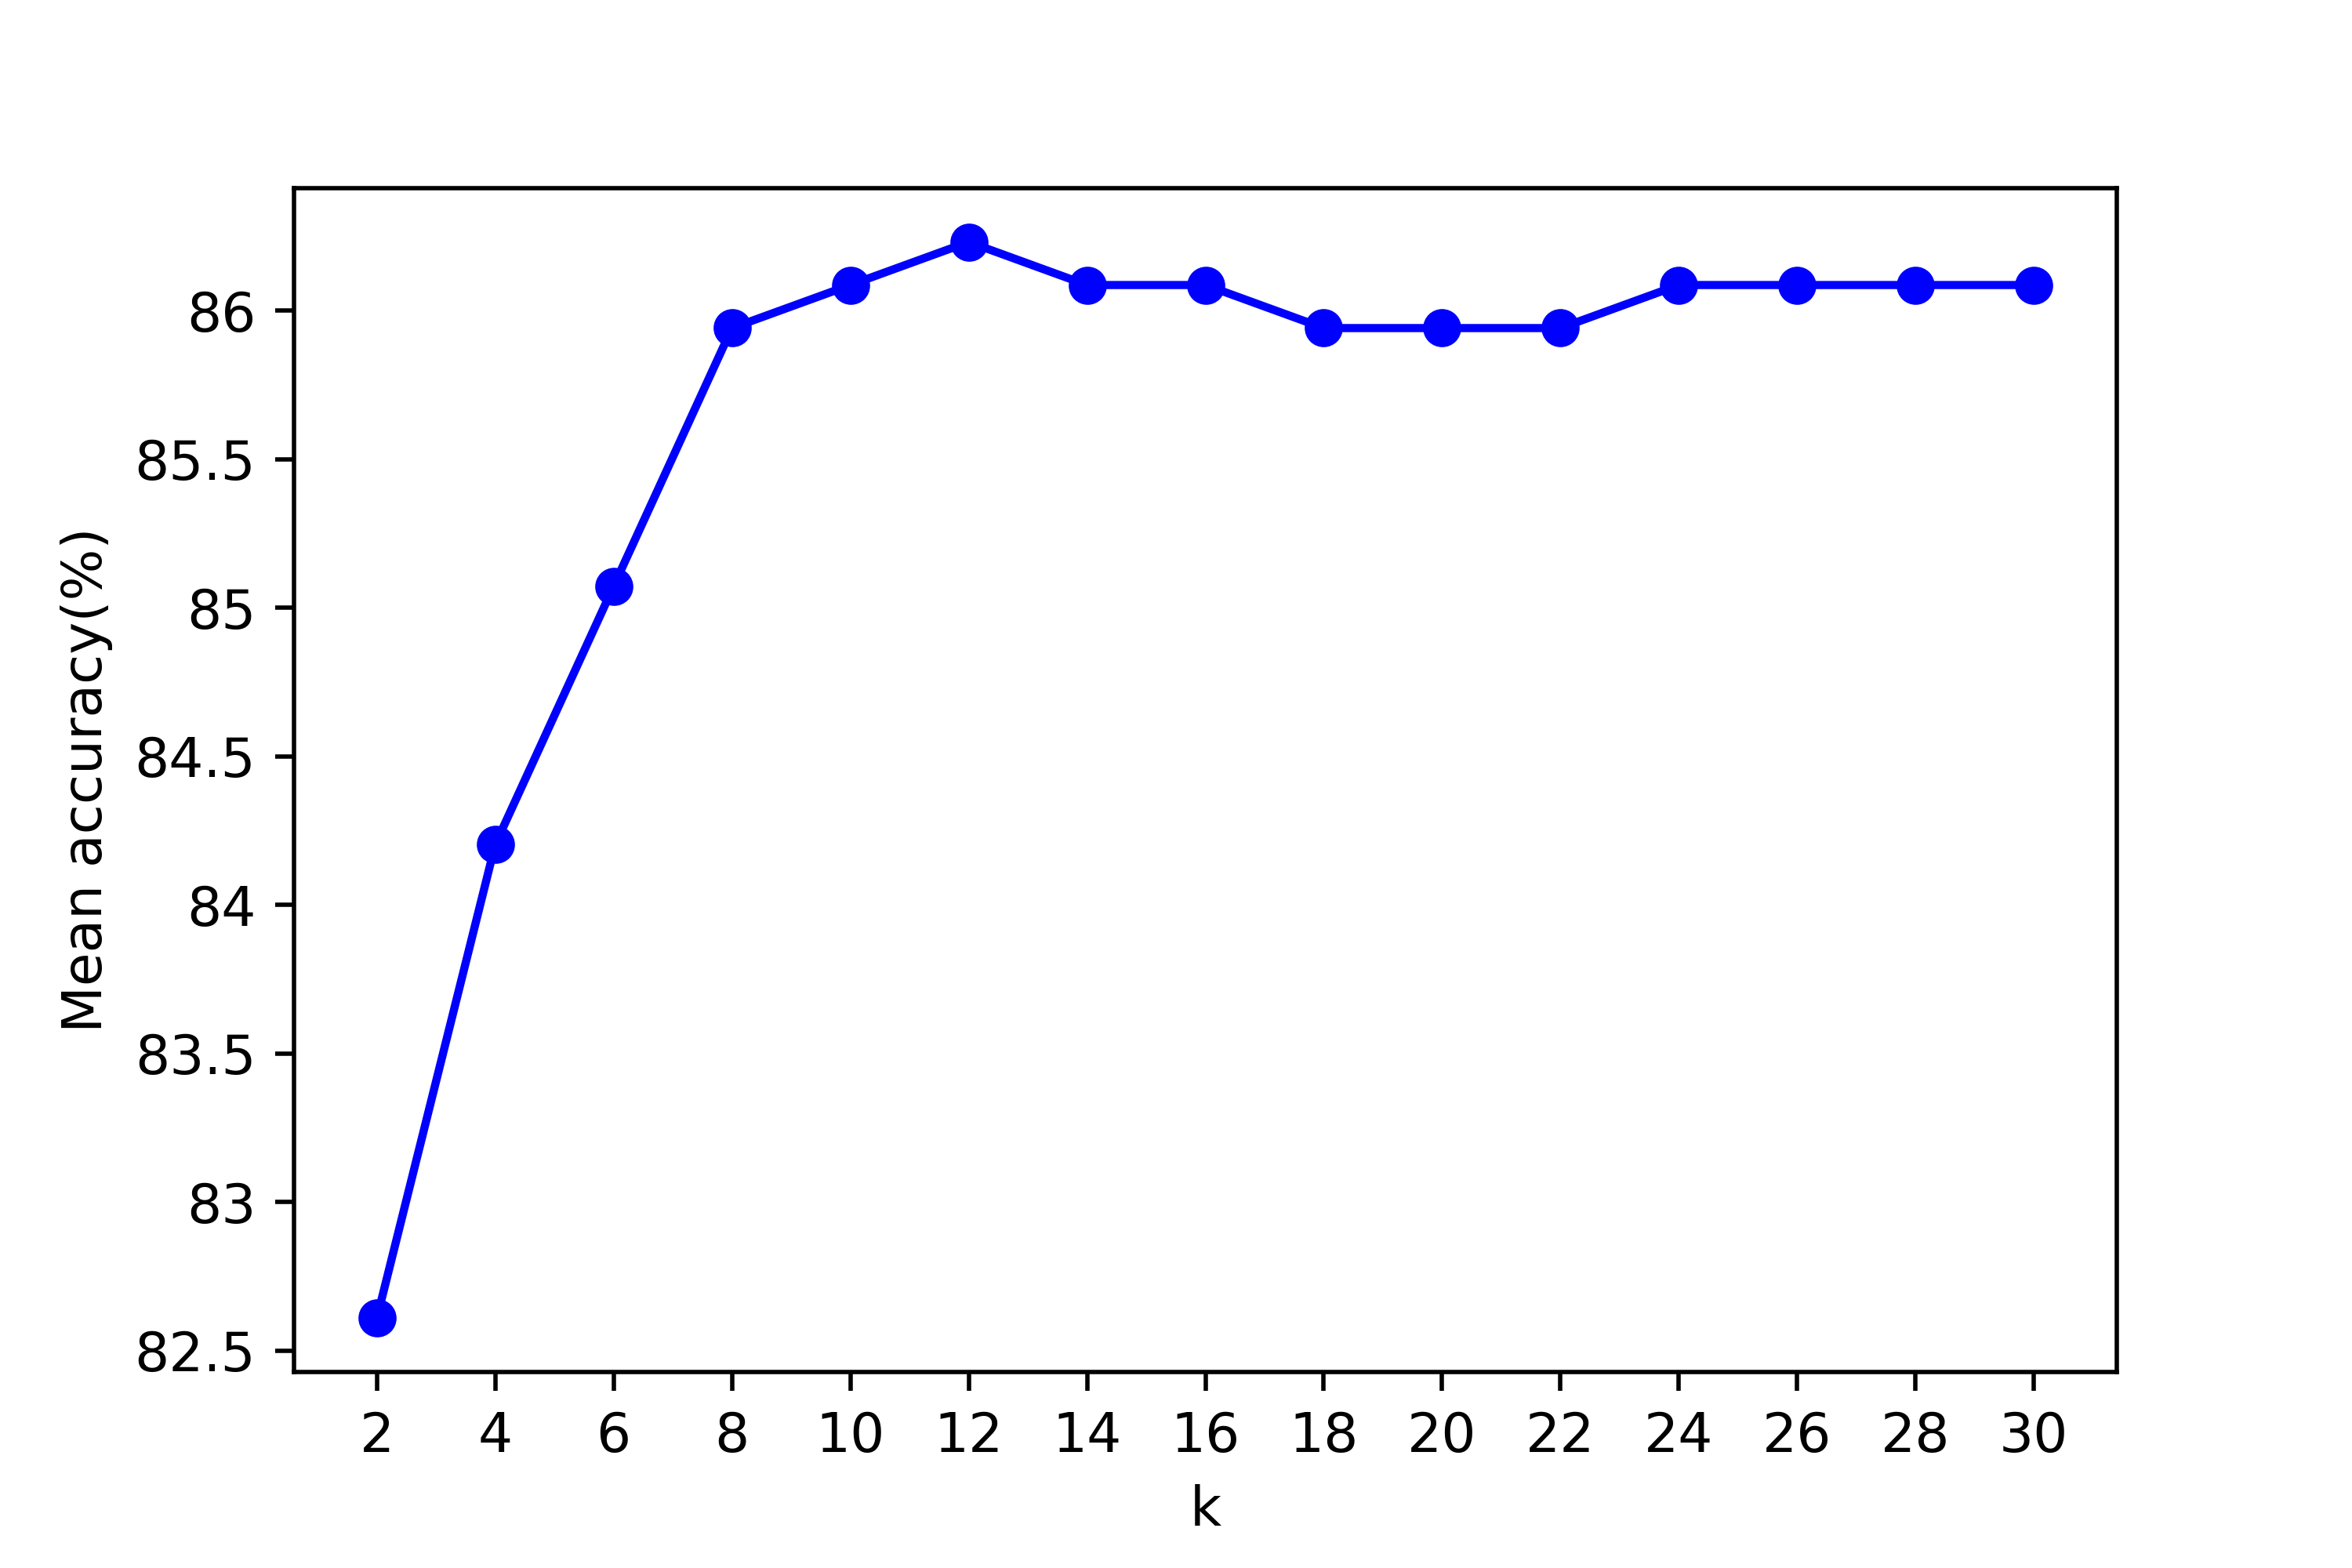
\includegraphics[width=0.5\textwidth]{KNN-LSTSVM-Aust}}
	\subfloat[مجموعه داده \lr{Hepatitis}]{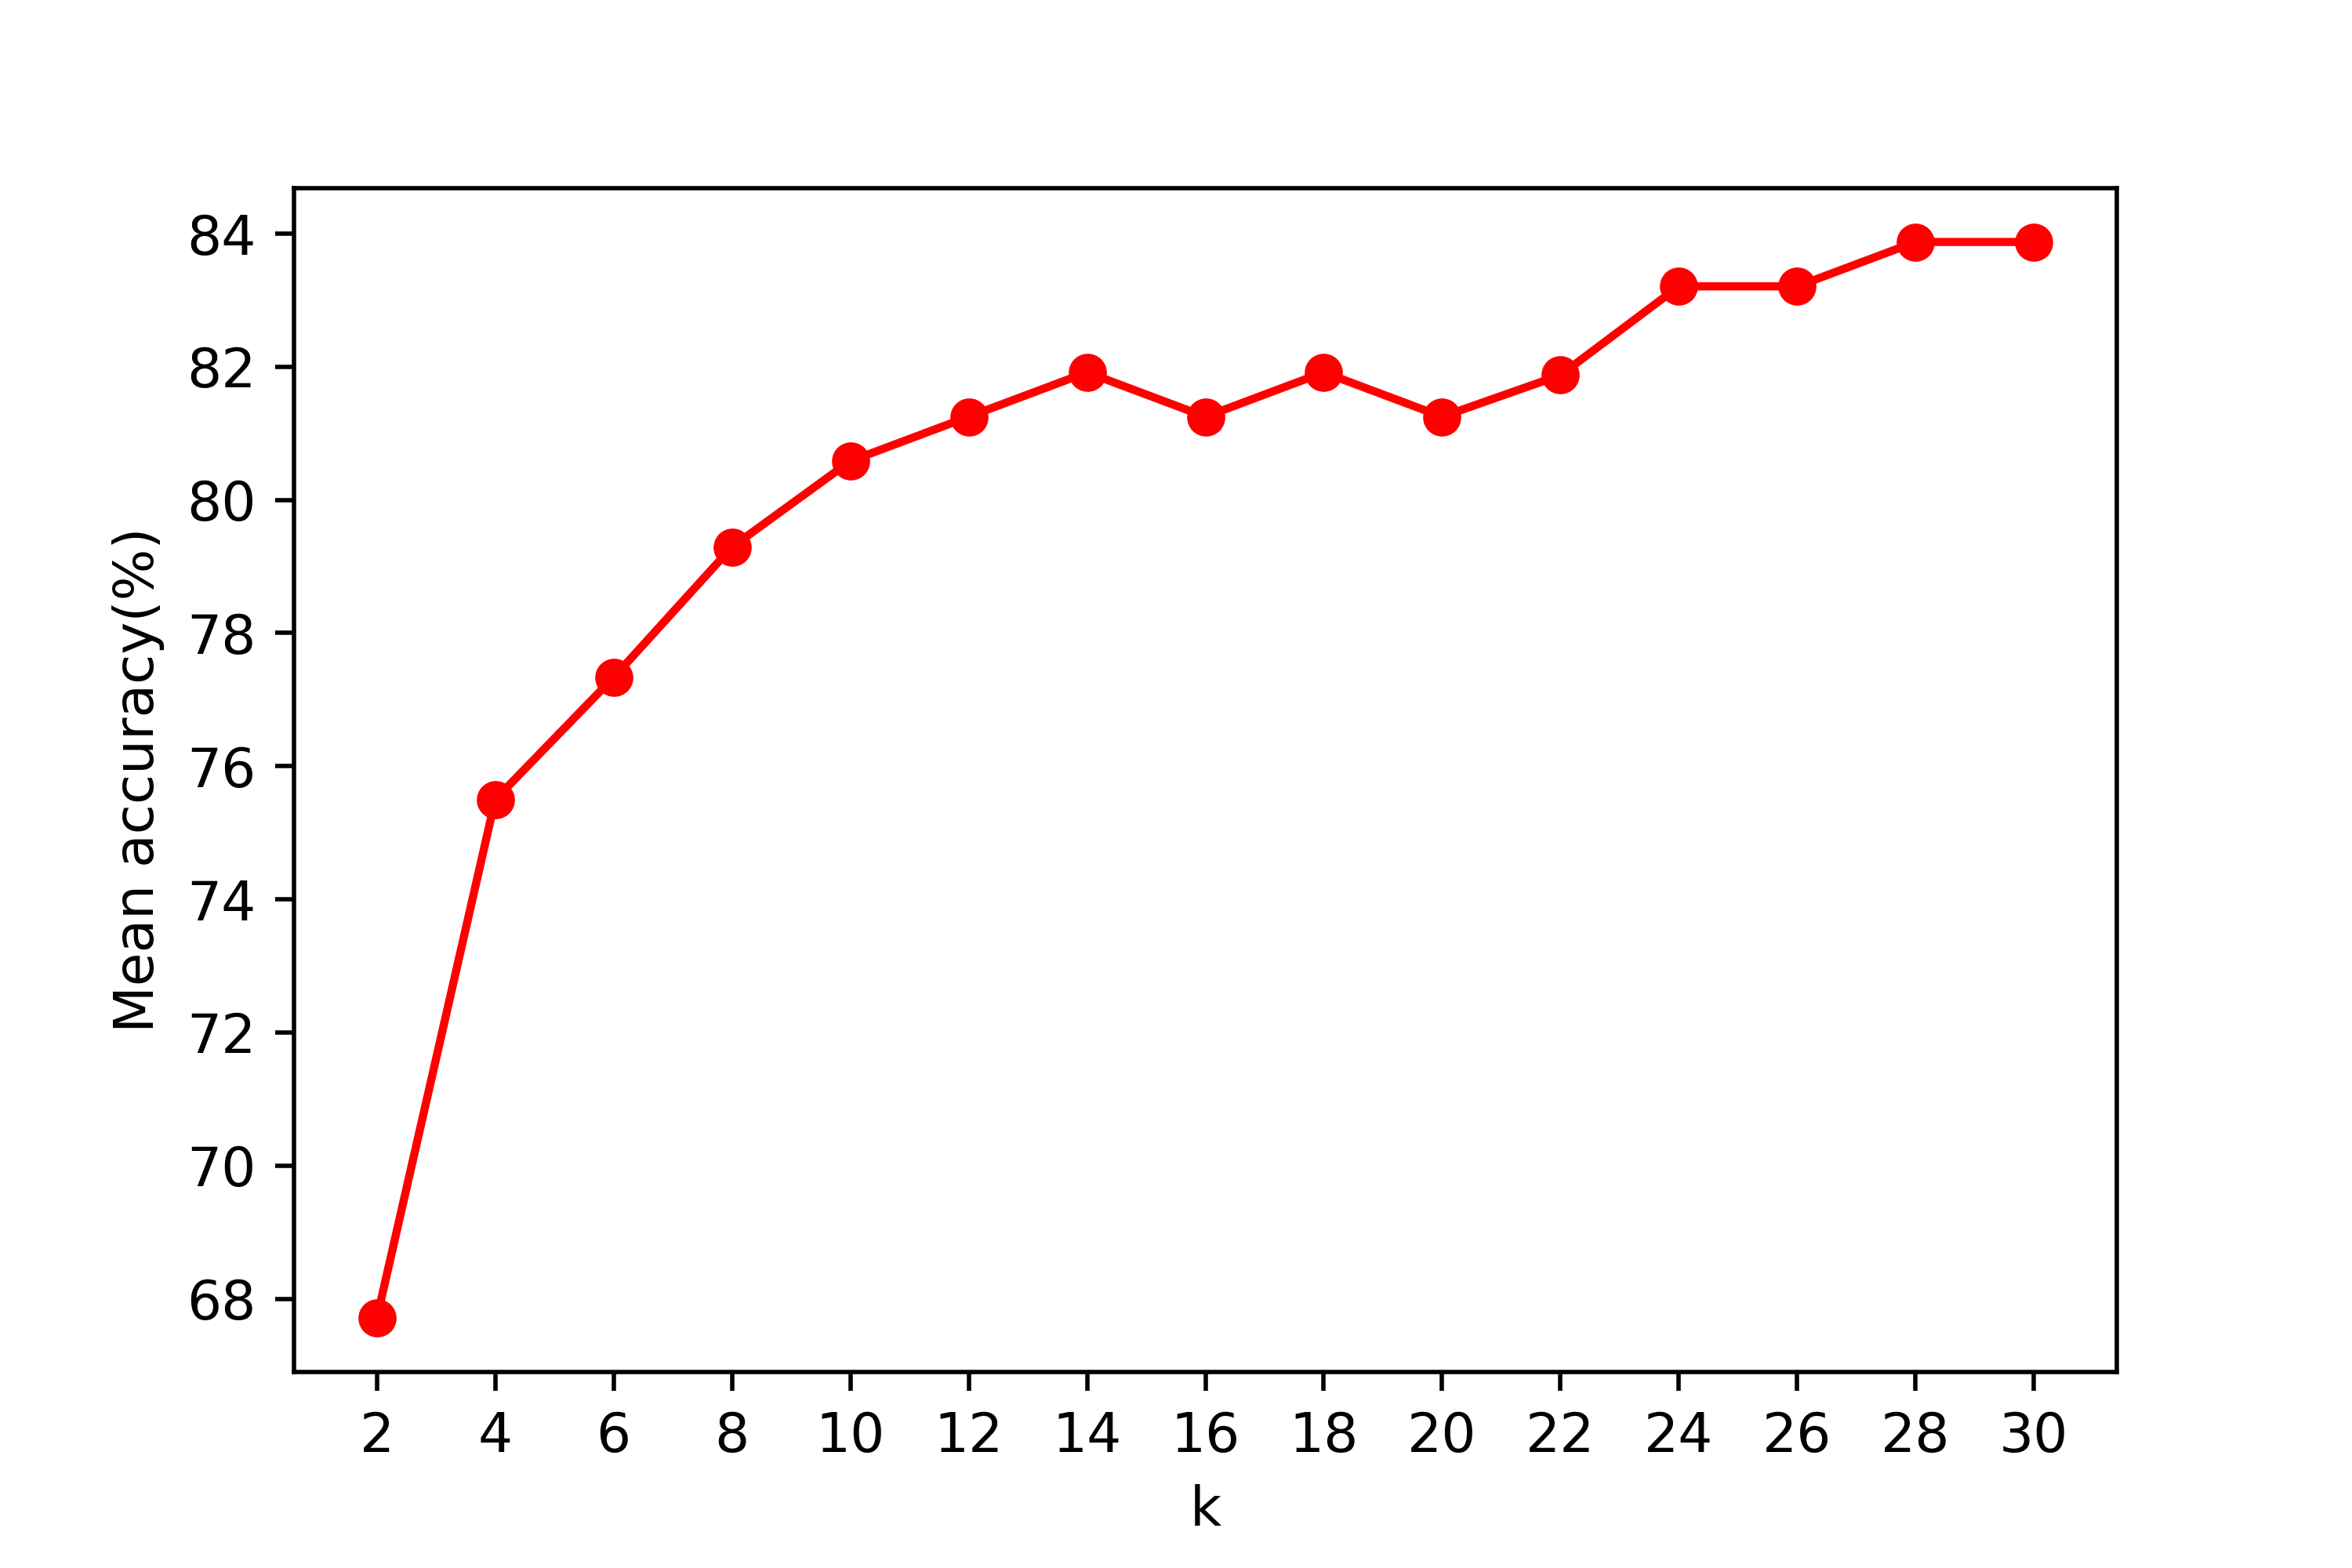
\includegraphics[width=0.5\textwidth]{KNN-LSTSVM-Hepa}}
	\caption{اثر افزایش پارامتر $k$ روی دقت دسته‌بند \lr{KNN-LSTSVM}}
	\label{fig:KNN-LSTSVM-Aust-Hepa}
\end{figure}

\subsubsection{بررسی آماری}\label{sec:5:2:3:1}
به منظور تحلیل بیشتر عملکرد چهار روش روی 14 مجموعه داده (جدول ‏5 2)، آزمون‌های آماری طبق پیشنهاد دمسار\footnote{\lr{Demsar}} \cite{demsar2006} استفاده می‌شود. بدین منظور آزمون آماری ساده و ناپارامتریک فریدمن\footnote{\lr{Friedman}}  مورد استفاده قرار گرفته است. به منظور انجام آزمون آماری، میانگین رتبه چهار روش بر اساس دقت محاسبه شده و در جدول ‏5 3 نشان داده شده است. ابتدا بر اساس فرض صفر، تمام روش‌ها را یکسان در نظر می‌گیریم. سپس آزمون فریدمن با رابطه زیر محاسبه می‌شود.
\begin{equation}\label{eq:5:1}
\chi^2_F = \frac{12N}{k(k + 1)}\bigg[\sum_{j} R^2_j - \frac{k(k + 1)^2}{4} \bigg],
\end{equation}

در رابطه \ref{eq:5:1}،  $R_j=\frac{1}{N}\sum_{i}r^j_i$ و $r_{i}^{j}$  نشان‌دهنده رتبه $j$مین روش بر روی $i$مین مجموعه داده از  $N$ است. 

\begin{table}[!t]
	\centering
	\caption{میانگین رتبه براساس دقت (ارزیابی \lr{KNN-LSTSVM})}
	\ra{1.3} % Space between rows
	\tabcolsep=0.10cm
	\begin{tabular}{c c c c c c c c c c c c}
		\toprule
		% after \\: \hline or \cline{col1-col2} \cline{col3-col4} ...
		مجموعه داده & \lr{TSVM} & \lr{WLTSVM} & \lr{LSTSVM} & \lr{KNN-LSTSVM} \\
		\midrule
	\lr{Austrailian} & 1 & 4 & 2 & 3\\
	\lr{Bupa-Liver} & 4 & 2 & 3 & 1\\
	\lr{Cleveland} & 3 & 4 & 2 & 1\\
	\lr{Haber-Man} & 3 & 4 & 2 & 1\\
	\lr{Heart-Statlog} & 1 & 3 & 3 & 3\\
	\lr{Hepatits} & 4 & 3 & 1 & 2\\
	\lr{Ionsphere} & $1.5$ & 3 & 4 & $1.5$\\
	\lr{Monk3} & 4 & 3 & 2 & 1\\
	\lr{Pima-Indian} & 2 & 3 & 4 & 1\\
	\lr{Sonar} & 3 & 1 & 4 & 2\\
	\lr{Titanic} & 3 & 4 & 1 & 2\\
	\lr{Votes} & 4 & $2.5$ & 1 & $2.5$\\
	\lr{Wdbc} & 1 & 4 & 2 & 3\\
	\lr{Wpbc} & 2 & 4 & 3 & 1\\
	میانگین رتبه & $2.61$ & $3.18$ & $2.43$ & \textbf{$1.79$} \\
		\bottomrule
	\end{tabular}
	
	\label{tab:6}
\end{table}

سپس مقدار $F_F$  براساس  $\chi^2_F$ به صورت زیر محاسبه می‌شود. بطوریکه $F_F$ از توزیع $F$ با $(k-1)$ و $(k-1)(N-1)$ درجه آزادی پیروی می‌کند.
\begin{equation}\label{eq:5:2}
F_F = \frac{(N - 1)\chi^2_F}{N(k - 1) - \chi^2_F}
\end{equation}

بر اساس روابط \ref{eq:5:1} و \ref{eq:5:2}، مقادیر $\chi^2_F = 8.293$ و  $F_F = 3.198$ بدست آمده است. در اینجا $F_F$ از توزیع $F$  با (39، 3) درجه آزادی پیروی می‌کند. مقادیر ویژه $F(3, 39)$ برای سطوح معناداری 25/0، 1/0 و 05/0 به ترتیب برابر  42/1، 23/2 و 84/2 است. مقدار  $F_F$ به طور قابل توجه‌ای بیشتر از مقدار ویژه است. بنابراین از آزمون آماری استنتاج می‌شود که تفاوت قابل توجه‌ای بین 4 روش وجود دارد. همچنین جدول ‏\ref{tab:6} نشان می‌دهد که روش پیشنهادی (\lr{KNN-LSTSVM}) در مجموع عملکرد بهتری نسبت به سایر روش‌ها دارد. زیرا میانگین رتبه روش پیشنهادی در میان سایر روش‌ها کمترین است.

\subsection{مجموعه داده \lr{NDC}}\label{sec:5:2:4}


\newpage

\section{ارزیابی روش \lr{RKNN-TSVM}}\label{sec:5:3}
